\section{Algorithm}
\label{Algorithm}

The algorithm we are presenting works on two main steps:
\begin{itemize}
  \item Build the data structure - the efficiency of the algorithm is determined by the data structure it runs on. On the other hand, the data structure is specifically designed to solve this problem.
  \item Traverse data structure and output result - the algorithm works by looping through all the actors and finding the most promising connections.
\end{itemize} 

\subsection{Notations}
Let G = (V,E) be a weighted, directed simple graph and let n = \(\lvert V\rvert\) and m = \(\lvert E\rvert\).

A vertex v denotes an actor. Any edge e between vertices \(v_1\) and \(v_2\) denotes a set of movies these two actors have played together. Weight of the edge, W(e) denotes the size of that set. An edge is always directed from the actor with lower Id to the actor with higher Id.

Denote by A(v) the set of adjacent edges to vertex v.

SET(e) is the set of (two) vertices adjacent to an edge e.

Unique(\(v_1, v_2,... v_n)\) - returns a set of unique elements.

MovieCount denotes the biggest number found so far of common movies between any given three actors.

\subsection{Data structure}
As mentioned in the previous section, the algorithm starts by first building the data structure. The data structure is a graph, where vertices represent actors and edges between them represent the movie(s) these actors played together in. 

\begin{figure}[ht!]
\centering
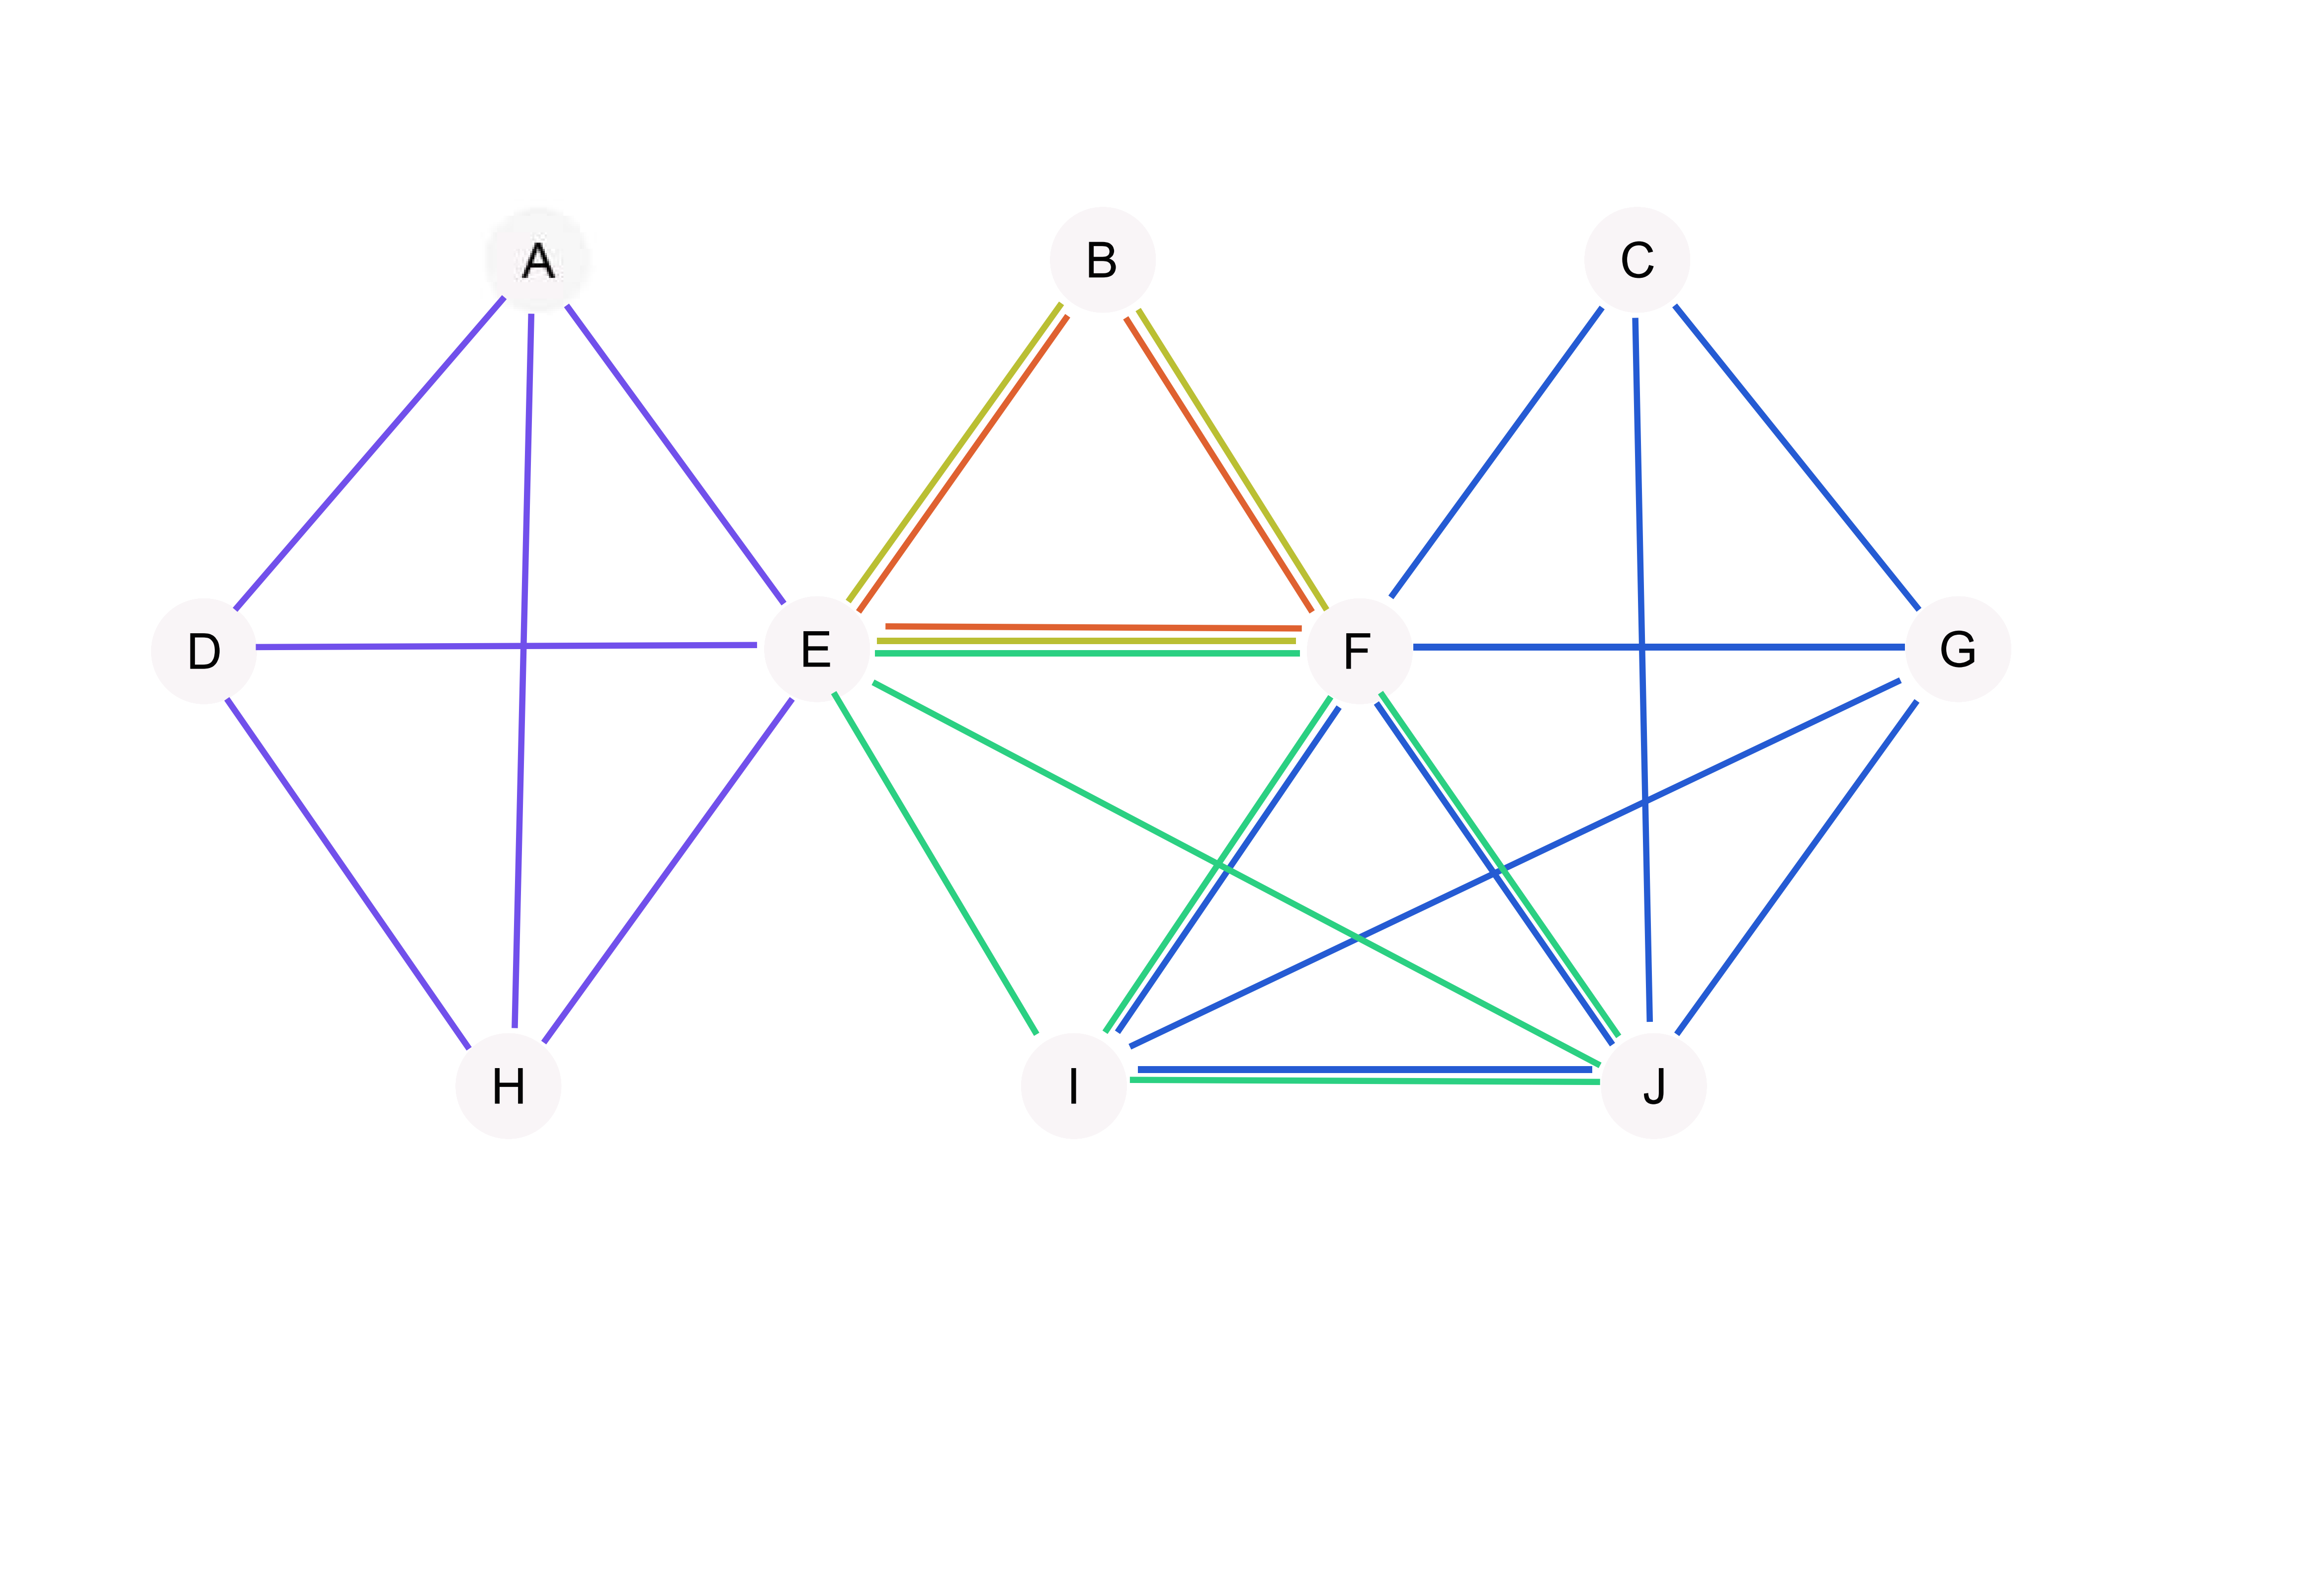
\includegraphics[width=130mm]{resources/project_problem_illustration.png}
\caption{Graph Example}
\label{example}
\end{figure}

Figure \ref{example} represents the data structure. To clearly illustrate the problem, the picture above represents a multi-graph, i.e. there can be multiple edges between two vertices. This is not the case of the actual data structure, however, as multiple edges are collapsed into a single one, where the weight is the sum of the weights of the original edges. The weight of an edge is the initially 1 - a single movie common to two actors (vertices). The edge contains sorted list of the movies common for two actors adjacent to the specific edge.
\\
After the structure is constructed, the actual data processing takes place.


\subsection{Pseudocode}
Main algorithm we implemented is FindThreeActors. After constructing the graph, we iterate over all vertices (actors). We find for each vertex all subsets of size of two of the set of adjacent edges to that vertex. We take an advantage of the fact that if an actor 1 played together in the same movie "A" with an actor 2 and the actor 1 played together with an actor 3 in the movie "A", that means that the actor 2 and the actor 3 had to play together in the movie "A". So we decided not to look for triangles in traditional way, but we look for pairs of edges having movies in common being adjacent to a specific vertex.
\\
We examine each pair of edges and we find the number of common movies that actors played in together (this is a common set of the subsets - the movies from two edges).  We do that only if minimal weight of edges is higher than found (by now) maximum number of movies that actors played together. 
\\
If the solution is better that the already found, we save it. We continue searching and at the end, we remove any references to the adjacent edges to the analysed vertex. This will make future iterations faster, since less edges need to be examined. We go to the next iteration. 
\\
Pseudocode for the algorithm is presented below:

\begin{verbatim}
Algorithm 2: FindThreeActors(graph)
1	moviesCount ← 0;
2	{a1,a2,a3};
3	FOR v ∈ V DO
4	  FOR i ← 0 to size of A(v) DO
5	    e1←A(v)[i];
6	    IF MoviesCount < W(e1) THEN
7	      FOR j ← i + 1 to size of A(v) DO	          
8	          e2←A(v)[j];
9	          IF MoviesCount < W(e2) THEN
10	              count ← CommonMovieSubsetCount(e1, e2);
11	             IF moviesCount < count THEN
12	                  movieCount ← count;
13	                  {a1,a2,a3} ← Unique(SET(e1), SET(e2));
14	             END IF
15	          END IF
16	      END FOR
17	    END IF
18	  END FOR
19	END FOR
20	RETURN moviesCount, {a1,a2,a3};	  	                    	  
\end{verbatim}


We designed CommonMovieSubsetCount that returns number of items that are common in 2 subset given as arguments. We take advantage of the fact that the lists are sorted and we iterate over all the items in both lists in linear time. 
\\
The pseudocode is present below:

\begin{verbatim}
Algorithm 3: CommonMovieSubsetCount(movies1, movies2)
1	count ← 0;
2	p1 ← 0;
3	p2 ← 0;
4	WHILE p1 < W(movies1) AND p2 < W(movies2)
5	  IF movies1[p1] = movies2[p2] THEN
6	    INCREMENT(count);
7	    INCREMENT(p1);
8	    INCREMENT(p2);
9	  ELSE IF movies1[p1] < movies2[p2]
10	   INCREMENT(p1);
11	 ELSE IF movies1[p1] > movies2[p2]
12	  INCREMENT(p2);
13	END IF
14	RETURN count;
\end{verbatim}

\subsection{Parallelism}
\label{Parallelism}
Since the IMDB database is enormous and building graph for such an amount of data, requires lots of RAM, we wanted to split the problem and make computations on separate parts in parallel. We took care of not loosing any data and not processing any data more times than once. The other important thing was to split data into parts that require the same amount of work for CPU.
\\
Each separate group contains specific number of actors and edges coming out from them. The division is done by creating a list of edges (an edge contains 2 actors and a movie these 2 actors played together), where there is no repetition of edges (an edge is always directed from an actor with higher Id to an actor with lower Id). We sorted the list according to the Id of the first actor (in this actor with lower Id in an edge). We noticed that since an edge goes to the actor with higher Id, vertices with lower Ids have much more edges going out from it than getting in, so we could not just picked the first x actors from the list. 
\\
For instance if we want to have ten groups, to split data evenly in each group, we just picked every 10th vertex (actor) from the sorted list we have. That guaranties that workload on every part of data is similar, since each vertex has less and less edges coming out from it.
\\
We claim that we do not process same data multiple times. It is shown on the drawing \ref{triple}.

\begin{figure}[ht!]
\centering
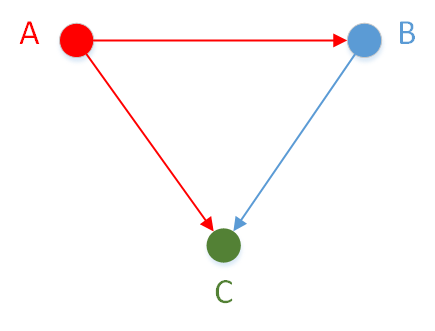
\includegraphics[width=90mm]{resources/triple.png}
\caption{Vertex Triple}
\label{triple}
\end{figure}

All three vertices are connected to each other and are placed in three different groups (red, blue and green). In group red we have a vertex A and two outgoing edges. In blue group we have a vertex B and one outgoing edge. In group green we have only vertex C without any outgoing edges. We can see that the presented triple will be analysed only once when we will process the vertex A in group red.
\\
The presented division allows us to run computations in parallel. Each thread results in a triple and number of movies actors played together in. After finishing computing all the data, we just need to aggregate the results and find the triple that played in the most number of movies. The figure \ref{threads} models the aggregation done by process 0 of the work produced by processes from 1 to n. In our case depth is 1 and work is n.


\begin{figure}[ht!]
\centering
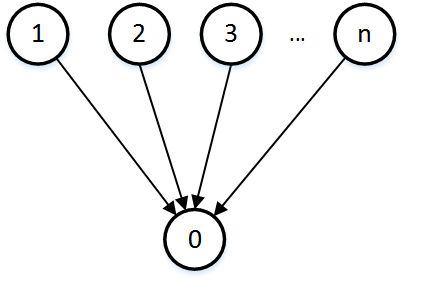
\includegraphics[width=90mm]{resources/threads.png}
\caption{Threads Work Aggregation}
\label{threads}
\end{figure}

We can run parallel computations on the same machine or on the separate machines. When we want to run it on the same machine, we have to consider amount of RAM the machine has and amount of parallel processes we can run on it.

\subsection{Analysis}
By not choosing to implement a traditional triangles counting O(\(n^3\)), we avoided to examine three times the same vertex. To do so, we constructed a special data structure and by consolidating edges, we saved used space to save the data.
In the worst case scenario, when each actor played together with another one (it is not realistic situation though) we will have n vertices and n*(n - 1)/2 edges.
\\
Complexity of the algorithm highly depends on degree of vertices. The higher it is, the longer computation time is required. It is related to the process of looking for subsets of size two for each vertex. The running time of the algorithm is \(\sum\limits_{i=1}^n{k_i \choose 2}\) where \(k_i\) is size of A(\(v_i)\), v \(\in\) V. The complexity of the algorithm counted for the worst case is calculated below. The worst case scenario is when an input for our algorithm is a full graph (all actors in the database played together).
\\
t(n,k) = \(\sum\limits_{i=1}^n{k_i \choose 2}\) \(\approx\) \(\sum\limits_{i=1}^n{k_i^2}\) \(\approx\) \(n*k_{max}^2\) \(\approx\) \(n*(n-1)^2\) = O(\(n^3\))
\\
Comparing our approach to Misra-Gries algorithm presented in chapter \ref{Standard}, we can see that the complexity of our algorithm is lower. We present differences in computation time in table \ref{comparison}. The values are counted for the worst case scenario, meaning the worst value we found in dataset. Let a be a constant and equals to 1274, that denotes the highest amount of actors played in a movie. Let k be a constant and equals to 15845. It is the highest number of adjacent vertices a vertex had found in database. Number of movies in IMDB equals to 388126 and number of actors equals to 817718. 
\begin{table}[ht]
\caption{Comparison of running times of Misra-Gries algorithm and our approach for the worst case scenario}
\centering
\begin{tabular}{c c c}
\hline\hline
Method & Running Time & Value \\ [0.5ex]
\hline
Misra-Gries&\(\sum\limits_{i=1}^m{a_i \choose 3}*h\)&\(4.805*e^{15} * h\)\\
Our approach&\(\sum\limits_{i=1}^n{k_i \choose 2}\)&\(4.106*e^{14}\)\\
\hline
\end{tabular}
\label{comparison}
\end{table}
The values obtained show that our approach has smaller time complexity than Misra-Gries. For the worst case scenario it is 10*h times.
\\
For the parallel approach, the running time is \(\sum\limits_{i=1}^n{k_i \choose 2}/x\) where x is number of threads and assuming that all the threads run simultanously. We ignore the time needed for aggregation after computing all the threads, since it is relatively small number.
